% Author: Rasmus Pank Roulund
% Inspired by figure in:
% Bebczuk, Ricardo N. (2003). Asymmetric Information in Financial
% Markets: Introduction and Applications. Cambridge University Press.

\documentclass{minimal}
\usepackage{tikz}
\usepackage{verbatim}

\begin{comment}
:Title: Asymmetric information

An illustration inspired by a figure in Bebczuk, Ricardo N. (2003). `Asymmetric Information in Financial Markets: Introduction and Applications. Cambridge University Press`__.

.. __: http://books.google.com/books?id=hYU_1v2BCWUC&dq=Asymmetric+Information+in+Financial+Markets:+Introduction+and+Applications&source=bn&ei=ATOXSceeH5KJ-ga0kMTvCA&sa=X&oi=book_result&resnum=4&ct=book-ref-page-link&cad=one-book-with-thumbnail

\end{comment}
\usetikzlibrary{arrows,calc}
\tikzset{
%Define standard arrow tip
>=stealth',
%Define style for different line styles
help lines/.style={dashed, thick},
axis/.style={<->},
important line/.style={thick},
connection/.style={thick, dotted},
}
\newcommand\A{\ensuremath{\mathcal{A}}}
\newcommand\B{\ensuremath{\mathcal{B}}}
\begin{document}

  \begin{tikzpicture}[scale=1.2]
    %Draw axis
    \coordinate (y) at (0,5);
    \coordinate (x) at (5,0);
    \draw[axis] (y) -- (0,0) --  (x);
    %Important coordinates. These are used in both figures and can be
    %moved to a seperate settings files
    %% These coordinates deside where boxes start on the y axis
    \coordinate (alphaas) at ($0.8*(y)$);
    \coordinate (alphabs) at ($0.533*(y)$);
    %% These coordinates deside where boxes end on the x axis
    \coordinate (cfas) at ($.6*(x)$);
    \coordinate (cfbs) at ($.9*(x)$);
    %These sets the interest rate lines 
    \coordinate (rl) at ($(cfas)-.2*(x)$);
    \coordinate (rla) at ($(rl)-.1*(x)$);
    \coordinate (rlb) at ($(rl)+.1*(x)$);
    %%%%%%%%%%%%%%%%%%%%%%
    %We makes some boxes and connect some coordinates
    %%%%%%%%%%%%%%%%%%%%%%
    %First, let us draw a line connecting alpha^\A_s og NV^\A_s
    \draw[important line] let \p1=(alphaas), \p2=(cfas) in 
    (\p1) node[left] {$\alpha_s^\A$} -| (\x2, \y1) -| (\p2)
    node[below] {$\mathit{NV^\A_s}$};
    %Second, let us connect alpha^\B_s og NV^B_s
    \draw[] let \p1=(alphabs), \p2=(cfbs) in 
    (\p1) node[left] {$\alpha_s^\B$} -| (\x2, \y1) -| (\p2)
    node[below] {$\mathit{NV^\B_s}$};
    %A line seperating the boxes.
    \draw[help lines] let \p1=(rl), \p2=(y) in
    (\p1) node[below] {$\hat{r}_L$} -- (\x1, \y2);
    %%%%%%%%%%%%%%%%%%%%%%
    %The small boxes will be assinged letter
    %%%%%%%%%%%%%%%%%%%%%%
    %%C
    \draw let \p1=($(alphaas)-(alphabs)$), \p2=(rl), \p3=(alphabs) in
    ($(.5*\x2, .5*\y1+\y3)$) node {$C$};
    %%D
    \draw let \p1=($(alphaas)-(alphabs)$), \p2=($(cfas)-(rl)$),
    \p3=(alphabs), \p4=(rl) in
    ($(.5*\x2+\x4, .5*\y1+\y3)$) node {$D$};
    %%E
    \draw let \p1=(alphabs), \p2=(rl) in
    ($(.5*\x2, .5*\y1)$) node {$E$};
    %%F
    \draw let \p1=(alphabs), \p2=($(cfas)-(rl)$), \p3=(rl) in
    ($(.5*\x2+\x3, .5*\y1)$) node {$F$};
    %%G
    \draw let \p1=(alphabs), \p2=($(cfbs)-(cfas)$), \p3=(cfas) in
    ($(.5*\x2+\x3, .5*\y1)$) node {$G$};
  \end{tikzpicture}
\quad
  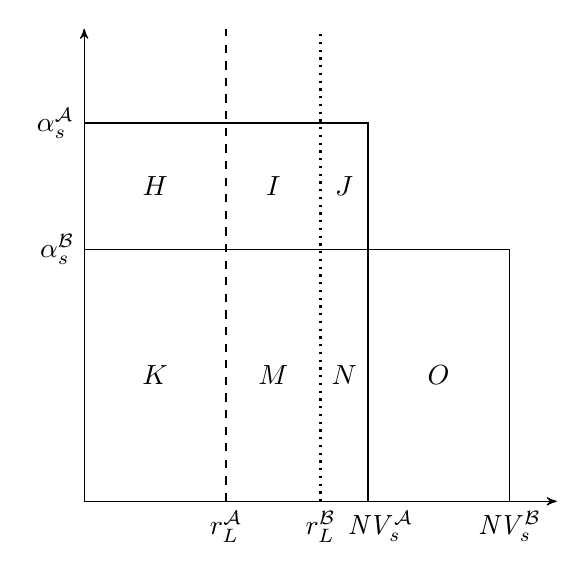
\begin{tikzpicture}[scale=1.2]
    %Axis
    \coordinate (y) at (0,5);
    \coordinate (x) at (5,0);
    \draw[axis] (y) -- (0,0) --  (x);
    %Important coordinates. These are used in both figures and can be
    %moved to a seperate settings files
    %% These coordinates deside where boxes start on the y axis
    \coordinate (alphaas) at ($0.8*(y)$);
    \coordinate (alphabs) at ($0.533*(y)$);
    %% These coordinates deside where boxes end on the x axis
    \coordinate (cfas) at ($.6*(x)$);
    \coordinate (cfbs) at ($.9*(x)$);
    %These sets the interest rate lines 
    \coordinate (rl) at ($(cfas)-.2*(x)$);
    \coordinate (rla) at ($(rl)-.1*(x)$);
    \coordinate (rlb) at ($(rl)+.1*(x)$);
    %%%%%%%%%%%%%%%%%%%%%%
    %We makes some boxes and connect some coordinates
    %%%%%%%%%%%%%%%%%%%%%%
    %First, let us draw a line connecting alpha^\A_s og NV^\A_s
    \draw[important line] let \p1=(alphaas), \p2=(cfas) in 
    (\p1) node[left] {$\alpha_s^\A$} -| (\x2, \y1) -| (\p2)
    node[below] {$\phantom{N}\mathit{NV^\A_s}$};
    %Second, let us connect alpha^\B_s og NV^B_s
    \draw[] let \p1=(alphabs), \p2=(cfbs) in 
    (\p1) node[left] {$\alpha_s^\B$} -| (\x2, \y1) -| (\p2)
    node[below] {$\mathit{NV^\B_s}$};
    %%%%%%%%%%%%%%%%%%%%%%
    %Here we need two lines seperating the large boxes
    %%%%%%%%%%%%%%%%%%%%%%
     \draw[help lines] let \p1=(rla), \p2=(y) in
     (\p1) node[below] {$r^\A_L$} -- (\x1, \y2);    
     \draw[connection] let \p1=(rlb), \p2=(y) in
     (\p1) node[below] {$r^\B_L$} -- (\x1, \y2);
    %%%%%%%%%%%%%%%%%%%%%%
    %The small boxes will be assinged letter
    %%%%%%%%%%%%%%%%%%%%%%
    %%H
    \draw let \p1=($(alphaas)-(alphabs)$), \p2=(rla), \p3=(alphabs) in
    ($(.5*\x2, .5*\y1+\y3)$) node {$H$};
    %%I
    \draw let \p1=($(alphaas)-(alphabs)$), \p2=($(rlb)-(rla)$),
    \p3=(alphabs), \p4=(rla) in
    ($(.5*\x2+\x4, .5*\y1+\y3)$) node {$I$};
    %%J
    \draw let \p1=($(alphaas)-(alphabs)$), \p2=($(cfas)-(rlb)$),
    \p3=(alphabs), \p4=(rlb) in
    ($(.5*\x2+\x4, .5*\y1+\y3)$) node {$J$};
    %%K
    \draw let \p1=(alphabs), \p2=(rla) in
    ($(.5*\x2, .5*\y1)$) node {$K$};
    %%M
    \draw let \p1=(alphabs), \p2=($(rlb)-(rla)$), \p3=(rla) in
    ($(.5*\x2+\x3, .5*\y1)$) node {$M$};
    %%N
    \draw let \p1=(alphabs), \p2=($(cfas)-(rlb)$), \p3=(rlb) in
    ($(.5*\x2+\x3, .5*\y1)$) node {$N$};
    %%O
    \draw let \p1=(alphabs), \p2=($(cfbs)-(cfas)$), \p3=(cfas) in
    ($(.5*\x2+\x3, .5*\y1)$) node {$O$};
  \end{tikzpicture}

\end{document}

%%% Local Variables: 
%%% mode: latex
%%% TeX-master: t
%%% End: 
